\documentclass{article}

\usepackage[utf8]{inputenc}
\usepackage[russian]{babel}
\usepackage{amsmath}
\usepackage{hyperref}
\usepackage{framed}
\usepackage{graphicx}
\renewcommand{\c}[2]{$C_{#1}^{#2}$}
\newcommand{\cc}[2]{C_{#1}^{#2}}

\newenvironment{exercise}{%
\begin{framed}\par\noindent\slshape%
}%
{\end{framed}}

\title{Поиск кратчайших расстояний в графе}
\author{}
\date{}

\begin{document}
\maketitle

\section{Алгоритм Дейкстры~--- поиск кратчайших расстояний от одной вершины до всех остальных.}

\begin{figure}
\begin{center}
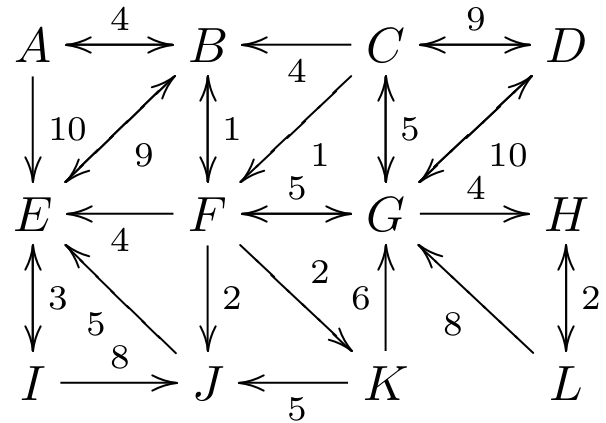
\includegraphics[width=0.5\textwidth]{dijkstra-statement.png}
\end{center}
\caption{Граф для применения алгоритма Дейкстры}
\label{fig:dijkstra-statement}
\end{figure}

Дан граф, на ребрах графа указаны числа, их можно называть «весами» ребер. Расстояние между вершинами~--- это минимальная возможная сумма весов ребер на пути между вершинами. Например, на рисунке~\ref{fig:dijkstra-statement} расстояние от $A$ до $E$ равно 9. Оно достигается на пути $ABFE$. Более очевидный прямой путь $AE$ дает большую сумму весов: 10.

Алгоритм Дейкстры позволяет найти расстояния от одной вершины до остальных. В данном примере мы будем искать все расстояния от вершины $J$. Приведем сначала полный протокол работы алгоритма, он изображен на рисунке~\ref{fig:dijkstra-answer}, после этого обсудим, как он получился.

\begin{figure}
\begin{center}
	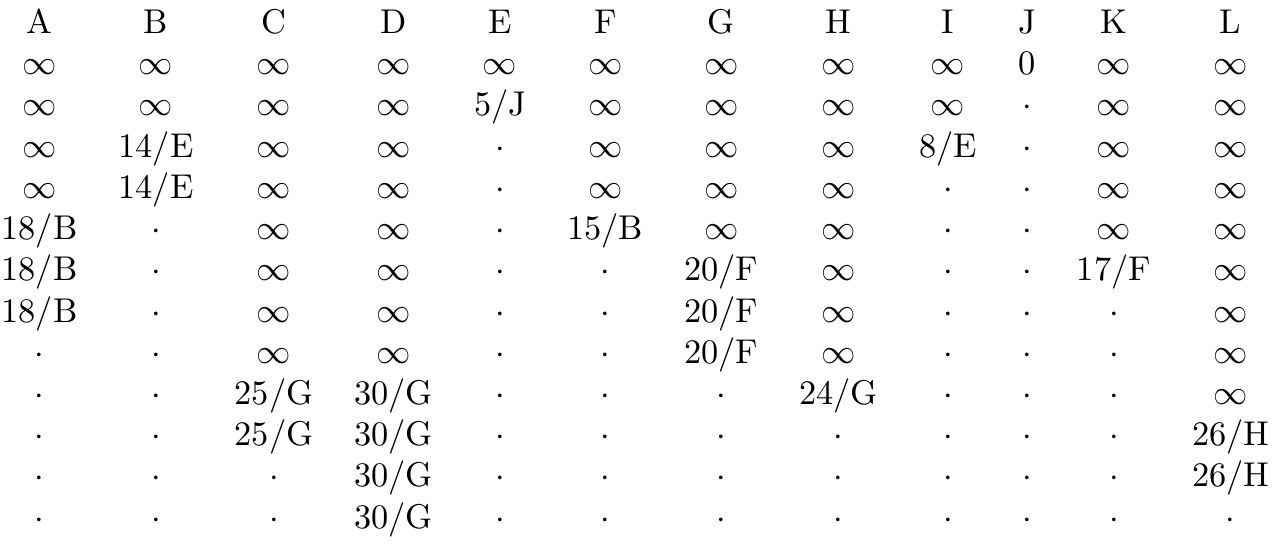
\includegraphics[width=\textwidth]{dijkstra-answer.png}
\end{center}
\caption{Протокол работы алгоритма Дейкстры}
\label{fig:dijkstra-answer}
\end{figure}

\subsection{Начало алгоритма}
В первой строке протокола выписаны все вершины. Мы будем писать под вершинами наши гипотезы о расстоянии до вершины $J$. Гипотезы будут постепенно улучшаться. Под названиями вершин выписываем начальные гипотезы о расстояниях. Расстояние до $J$, естественно, равно нулю, потому что мы с этой же вершины и начинаем путь. А расстояния до других вершин пока оценим как $+\infty$, пока ничего лучшего предположить невозможно.

\subsection{Как выписать очередную строку в протоколе}
Необходимо выбрать минимальное число в последней выписанной строке. У нас минимально выписан 0 в вершине $J$. Минимальное число является ответом для вершины. Для вершины $J$ совершенно неудивительно, что ответ 0. Больше в соответствующем столбце ставить числа мы не будем, в протоколе весь столбец дальше заполнен точками.

Теперь нужно проверить все ребра идущие из найденной вершины и попробовать улучшить по ним гипотезы до других вершин. Из вершины $J$ ведет только одно ребро: $JE$. Это значит, что мы можем попытаться улучшить путь до вершины $E$. Необходимо взять старое значение пути до $E$ из текущей строки, это $\infty$, и сравнить его с расстоянием до $J$ из текущей строки плюс вес ребра $JE$. Получается сравнение $\infty > 0 + 5$, это означает, что мы нашли более короткий путь до вершины $E$, равный пяти, это надо записать под вершиной $E$ в новой, второй строке с числами.

В этом примере протокола мы дополнительно записываем вершину, через которую произошло улучшение, т.е. например, пишем 5/J вместо 5, это нужно для восстановления оптимального пути. Но так как в ИДЗ оптимальный путь не спрашивается, можно при решении писать только длины пути без вершин.

Во второй строке чисел мы пишем точку под $J$, как объяснялось ранее, а для остальных вершин переносим значения из предыдущей строки.

Процесс продолжается дальше для каждой строки, пока не закончатся вершины.

\subsection{Пример выписывания четвертой строки снизу}

Рассмотрим еще, например, переход от пятой строки снизу к четвертой строки снизу.

В пятой строке снизу самое маленькое число~--- это 20 в вершине $G$. В остальных вершинах написано $\infty$ или ничего. Из $G$ ведут четыре ребра: $GC$, $GD$, $GF$, $GH$.

Рассмотрим ребро $GC$. Сравним текущее значение в вершине $C$, равное $\infty$ с расстоянием до $G$ плюс весом ребра $GC$. Это значит, сравним $\infty > 20 + 5$. Получается, произошло улучшение, и теперь наша гипотеза о расстоянии до вершины $C$~--- это 25. Запишем это в новую строку, четвертую снизу.

Расстояние до $D$ тоже улучшилось, это результат сравнения $\infty > 20 + 10$, где 20~--- это известное нам расстояние до $G$, а 10~--- вес ребра $GD$.

Ребро $GF$ нужно проигнорировать, потому что мы уже нашли ранее расстояние до $F$, равное 15, и теперь в соответствующем столбце можно ставить только пропуски. Но если желание проверить расстояние, можно сравнить текущее значение в $F$, равное 15 с суммой $20 + 5$, окажется, что текущее расстояние меньше, и заменять его не нужно.

Последнее, необходимо проверить ребро $GH$: $\infty > 20 + 4$, значит, в $H$ тоже произошло улучшение, и необходимо в вершине $H$ записать 24.

\section{Алгоритм Флойда~--- поиск кратчайших расстояний от каждой вершины до каждой}

\begin{figure}
	\begin{center}
		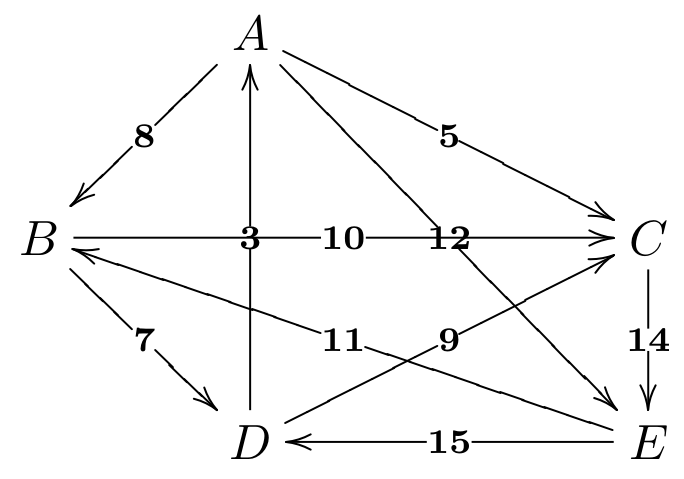
\includegraphics[width=0.5\textwidth]{floyd-statement.png}
	\end{center}
	\caption{Граф для применения алгоритма Флойда}
	\label{fig:floyd-statement}
\end{figure}

На рисунке~\ref{fig:floyd-statement} приведен граф, в котором мы будем считать расстояния от каждой вершины до каждой.

\subsection{Начальная матрица}
Рисунок~\ref{fig:floyd-answer} содержит протокол работы алгоритма. Слева сверху в нем находится начальная матрица расстояний~--- это матрица, в которой указаны веса ребер. Она строится напрямую по графу из условия задачи. Например, в условии изображено ребро $AB$ с весом 8, это значит, что в клетке в строке $A$ (т.е. в первой строке) и столбце $B$ (т.е. втором столбце) написано 8.
А, например, в строке $E$ (пятой), столбце $D$ (четвертом), написано 15, что соответствует ребру $ED$ веса 15.

\begin{figure}
	\begin{center}
		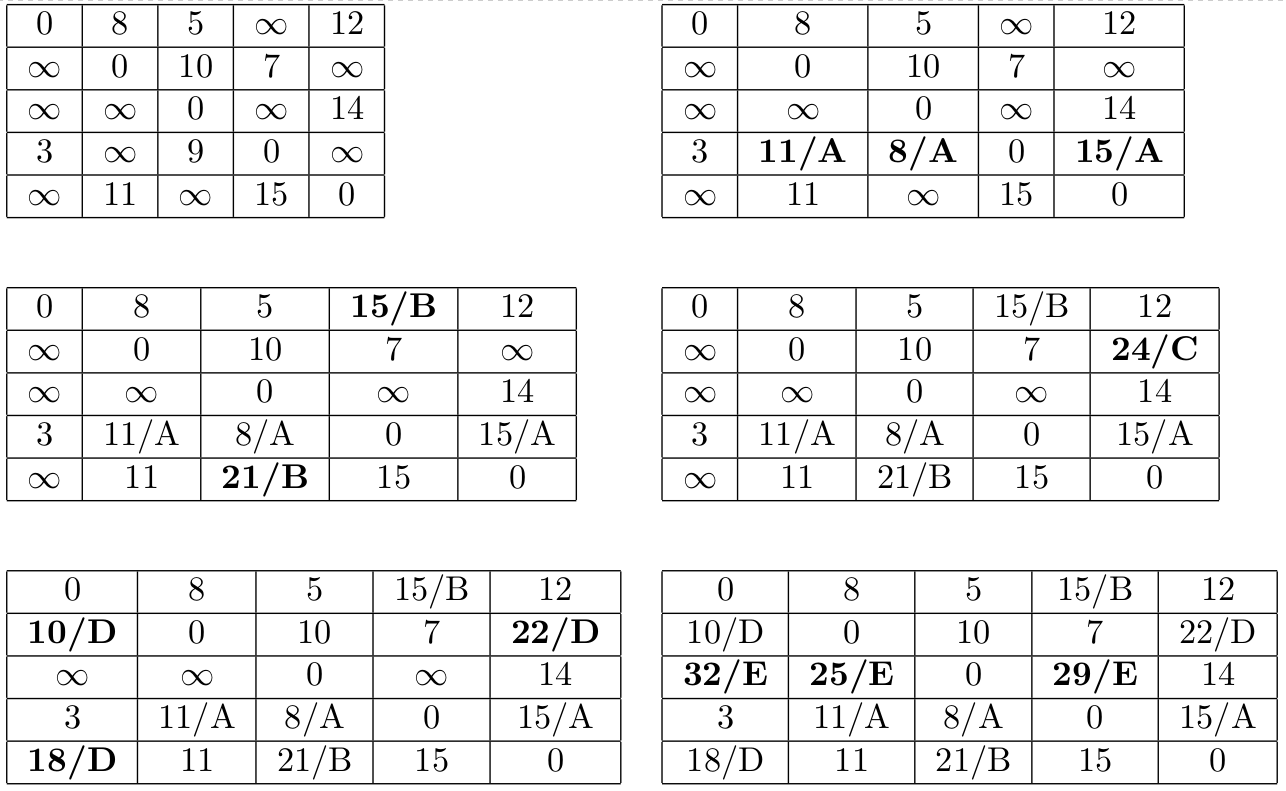
\includegraphics[width=\textwidth]{floyd-answer.png}
	\end{center}
	\caption{Протокол работы алгоритма Флойда}
	\label{fig:floyd-answer}
\end{figure}и

Фактически, начальная матрица~--- это матрица расстояний между вершинами, но при условии, что путь между вершинами не может содержать более одного ребра.
Соответственно, диагональ начальной матрицы всегда содержит 0. А если между какими-то вершинами ребра нет, в соответствующей клетке указывается $\infty$.

Убедитесь, что начальная матрица действительно соответствует графу, изображенному на рисунке~\ref{fig:floyd-statement}. После того, как эта матрица построена, исходный граф становится не нужен, все вычисления будут производиться только с матрицей.

\subsection{Если хотите запрограммировать алгоритм}
Интересной особенностью алгоритма Флойда является то, что он очень легко программируется. Если представить, что $a$~--- это начальная матрица, а $n$~--- количество вершин, то псевдокод выглядит следующим образом:

\begin{verbatim}
for k = 1 to n:
  for i = 1 to n:
    for j = 1 to n:
      if a[i, j] > a[i, k] + a[k, j]:
        a[i, j] = a[i, k] + a[k, j]
\end{verbatim}

Возможно, кому-то это объяснит, как работает алгоритм, и дальше можно будет не читать.

\subsection{Основной шаг алгоритма}

Алгоритму необходимо сделать несколько шагов, столько же, сколько вершин в графе. В нашем случае 5. На каждом шаге будет построена новая матрица. В приведенном на рисунке~\ref{fig:floyd-answer} протоколе как раз кроме начальной матрицы есть еще пять.

Каждый шаг соответствует какой-то вершине. Мы будем делать сначала шаг для вершины $A$, потом для вершины $B$ и т.д. по алфавиту.

Первый шаг, это обработка вершины $A$. Мы получим из исходной матрицы новую. Нужно перебрать все пары вершин, скажем, $XY$ и проверить, что меньше, исходное значение для пути от $X$ до $Y$, или значение пути от $X$ до $A$ плюс значение от $A$ до $Y$. Например, для клетки $DC$ (строка $D$, четвертая, и столбец $C$, третий) старое значение равно 9, а новое значение равно $DA + AC = 3 + 5 = 8$. Новое значение лучше, значит, нужно заменить в этой клетке число 9 на число 8.

Произведенные замены выделяйте, например, кружком. Здесь замены выделены жирным. Всего на шаге $A$ произойдет три замены, это замены для путей $DB$, $DC$, $DE$.

А вот число 7, например, для пути $BD$ заменено не будет. Потому что $BA + AD = \infty + \infty > 7$.

\subsection{Пример шага $D$}

На шаге $D$ мы строим матрицу, которая в протоколе нарисована слева снизу, из предыдущей матрицы справа посередине. Во всех вычислениях мы используем одну предыдущую матрицу, чтобы построить следующую. Более старые матрицы не нужны.

На этом шаге произойдут улучшения путей $BA$, $BE$, $EA$. Действительно, например, старое значение $BЕ$ это 24, а значение $BD + DE = 7 + 15 = 22$. Поэтому в соответствующей клетке 24 заменяется на 22.

\subsection{Некоторые оптимизации}
При построении очередной матрицы вы можете сразу заполнить диагональ нулями. Есть и другие оптимизации, которые могут помочь сократить вычисления.
Если вы находитесь на шаге $X$, то можете сразу переписать строки и столбцы с номером $X$, в них точно ничего не изменится. Например, на шаге $A$ можно сразу переписать из предыдущей матрицы первые строку и столбец.

Если вы на шаге, например $B$ видите, что клетка $CB$ содержит бесконечность, то всю строку $C$ можно оставить такой, какой она была. Дейстивтельно $CB + BX$ всегда будет равно бесконечности. Аналогично со столбцом. Если вы на шаге $B$ видите, что клетка $BE$ содержит бесконечность, то весь столбец $E$ можно переписать без изменений, так как $XB + BE = \infty$ и, значит, точно не приведет к улучшению.

\subsection{Ответ}

Ответом является последняя построенная матрица, которая получается после шага $E$. В ней указаны расстояния между всеми парами вершин. Так получается из-за основного свойства алгоритма. В начальной матрице у нас выписаны только прямые пути через одно ребро между всеми парами вершин. После шага $A$ мы учитываем пути, возможно, проходящие через $A$ в качестве промежуточной вершины. После шага $B$ мы учитываем пути, которые в качестве промежуточных вершин могут проходить через $A$ и через $B$. И т.д.

Кроме самой матрицы расстояний в условии задачи требуется восстановить конкретный путь. Например, давайте восстановим путь от $B$ до $E$. Он имеет длину 22. И мы знаем, что число 22 появилось в соответствующей клетке на шаге $D$. Для этого в протоколе при каждом улучшении значения рядом с ним появляется обозначение, на каком шаге это улучшение случилось. Следовательно, мы знаем, что оптимальный путь от $B$ до $E$ проходит через $D$. При этом мы не знаем пока, как устроен путь от $B$ до $D$ и от $D$ до $E$: $B {-?-} D {-?-} E$.

Проверим путь $BD$. В окончательной матрице видно, что этот путь ни разу не улучшался, значит оптимальный путь от $B$ до $D$~--- это ребро $BD$.

А вот путь от $D$ до $E$, равный 15, был улучшен на шаге $A$, значит, он проходит через вершину $A$. Итого, на данный момент мы понимаем, что путь устроен так: $B-D {-?-} A {-?-} E$. Но $DA$ и $AE$ ни разу не улучшались, значит, оптимальный путь между ними проходит по ребру. Окончательный ответ: путь от $B$ до $E$~--- это $B-D-A-E$ длины 22.

\end{document}